\input{doctools/latex/magazine_template.tex}   %Page setup
\input{doctools/latex/mycommands.tex}       %Some useful commands

% Figure search path
\graphicspath{
              {figs/} % Figures drawn with xfig
              {pngs/} % Other graphics files
}

% Use \draftnote to mark the filenames of figures
\newcommand{\isdraft}{1} %Choose 1 for draft, 0 for release

\begin{document}





%%%%%%%%%%%%%%%%%%%%%%%%%%%%%%%%%%%%%%%%%%%%%%%%%%%%%%%%%%%%%%%%%%%%
%Title
%%%%%%%%%%%%%%%%%%%%%%%%%%%%%%%%%%%%%%%%%%%%%%%%%%%%%%%%%%%%%%%%%%%%
\begin{center}
	{\huge ASCII command interface for the AVR Butterfly}\\
	\today
\end{center}

%%%%%%%%%%%%%%%%%%%%%%%%%%%%%%%%%%%%%%%%%%%%%%%%%%%%%%%%%%%%%%%%%%%%
%Table of contents
%%%%%%%%%%%%%%%%%%%%%%%%%%%%%%%%%%%%%%%%%%%%%%%%%%%%%%%%%%%%%%%%%%%%
\tableofcontents

\section{Introduction}
I love test equipment with open, well documented, ASCII command sets.  The plain text commands give a complicated-looking instrument a familiar interface, and beg you to use them in some clever measurement script.  Python's gnuplot and pySerial interfaces let you acquire and make pretty plots of your data -- all for free\cite{pyserial,gnuplot-py}. So when I need to automate hobby measurements at home, I immediately wish for an ASCII interface to whatever tool I'm measuring with.  This tool happens to be the AVR Butterfly board right now, simply because it's cheap and the LCD is handy.  

\clearpage
\section{Making connections to the Butterfly}
The AVR Butterfly board consists of an AVR ATmega169 microcontroller and some peripherals.  Figure \ref{fig:connections} shows the connections I make to it.  I only use 3 wires from the DB9 connector for serial communication with the PC -- there's no hardware handshaking.  And while I could also use this serial channel for programming, I find that using a dedicated programmer makes iterating my code much faster.  I thus solder a 6-pin header to the J403 position to use Atmel's AVRISP mkII programmer.  Finally, powering the board with an external supply at J401 means that I don't have to think about the Butterfly's button cell battery.

\begin{figure}[ht]
    \begin{center}
        \includegraphics[clip,scale=1]{usart_pinout}
        \draftnote{usart\_pinout.fig}
        \caption{Connections needed for the AVR Butterfly.\label{fig:connections}}
    \end{center}
\end{figure}

\clearpage
\section{Handling incoming characters}

\begin{figure}[ht]
    \begin{center}
        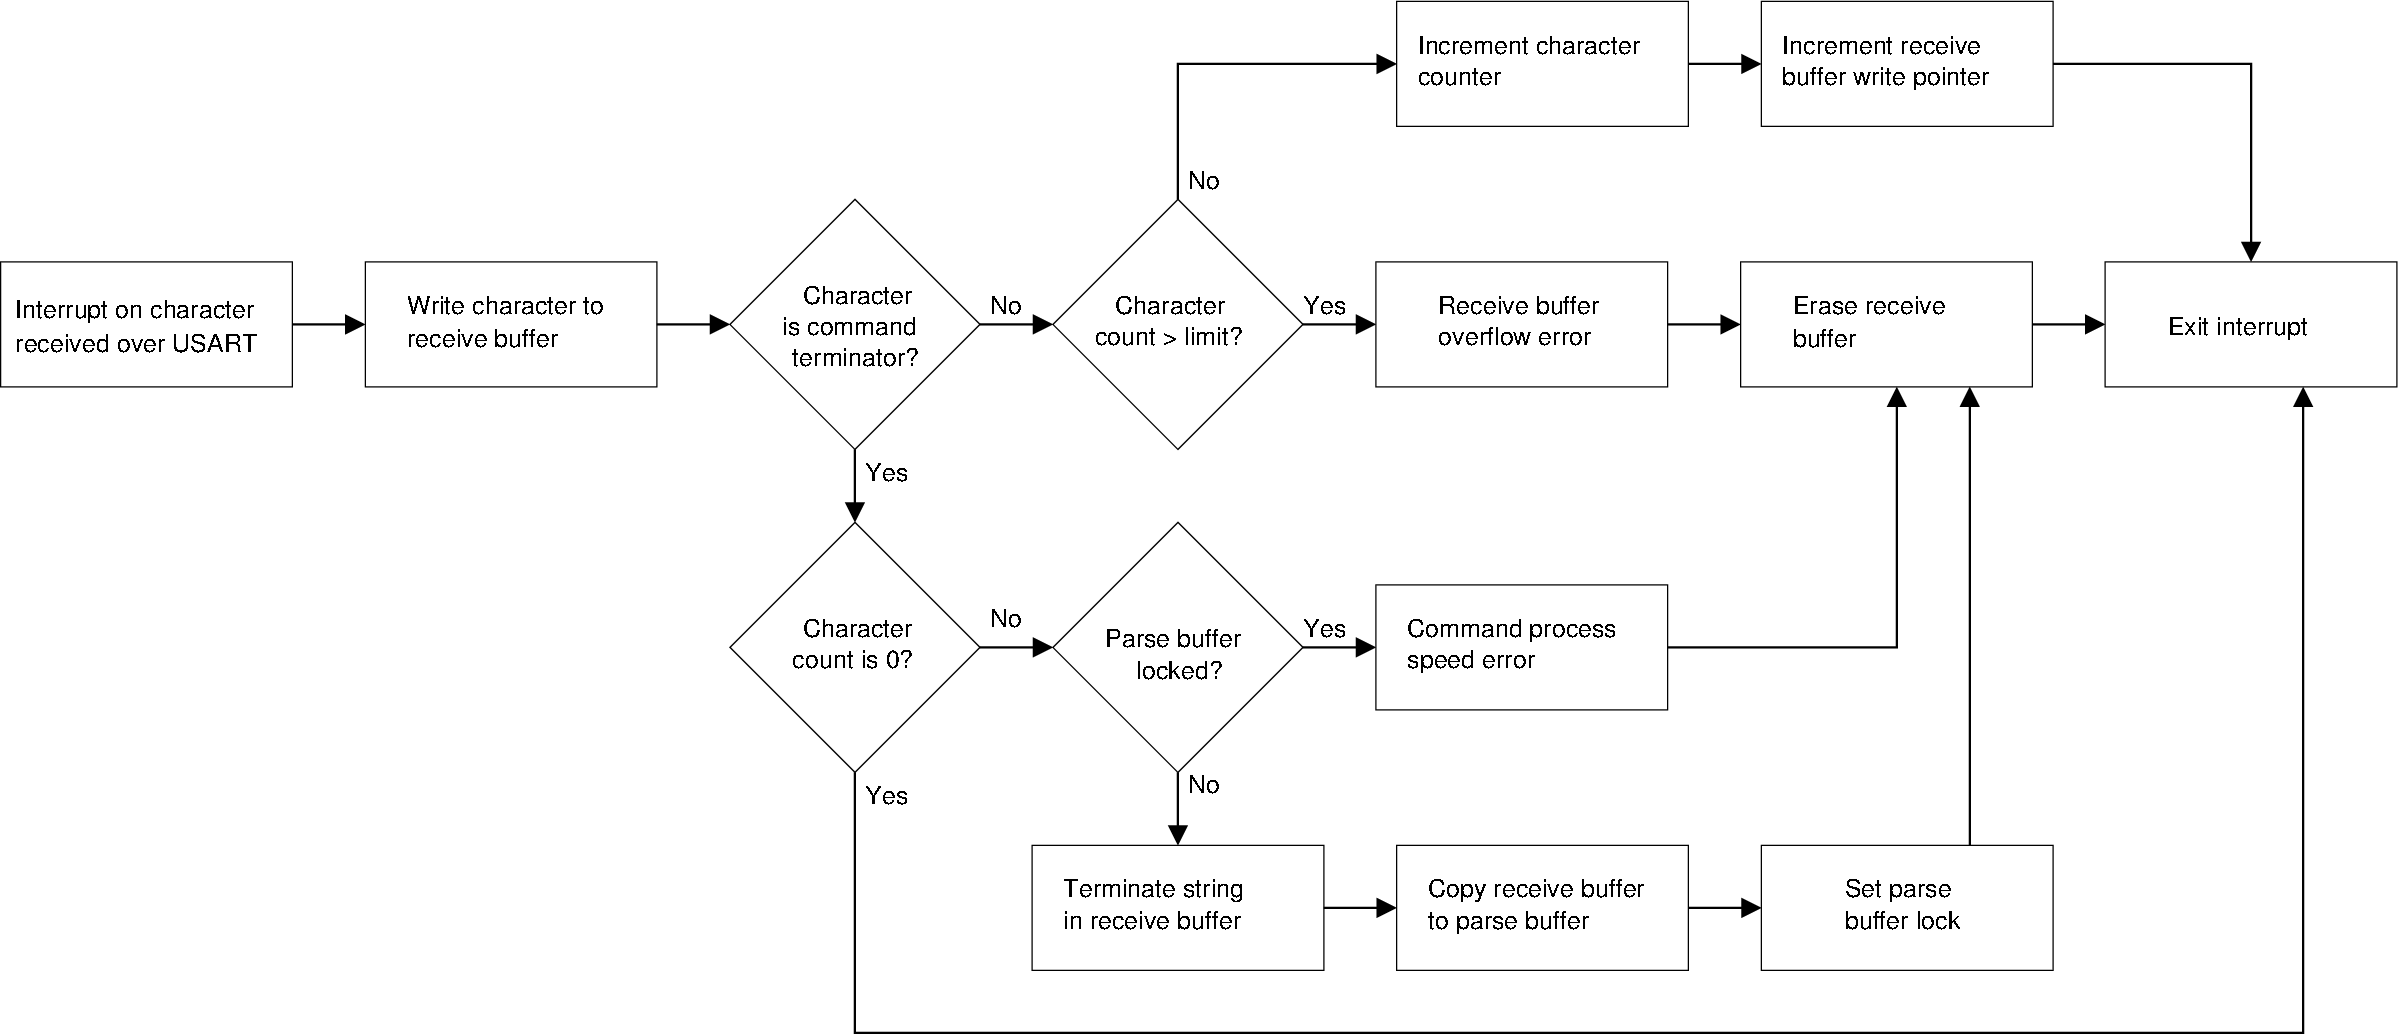
\includegraphics[clip,scale=0.45]{recv_cmd_flow}
        \caption{Program flow for processing characters received over the Butterfly's USART.\label{fig:recflow}}
    \end{center}
\end{figure}

\clearpage{}
\section{The debug output}

% See the termgrab.sh script for details about creating grab.eps
\begin{figure}[ht]
    \begin{center}
        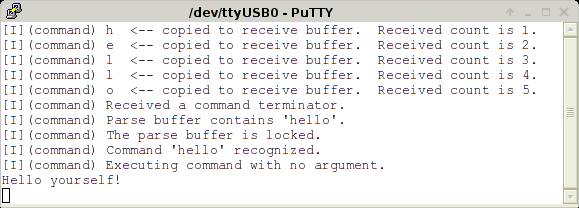
\includegraphics[clip,scale=0.5]{grab.eps}
        \caption{Terminal output showing debug information.\label{fig:termgrab}}
    \end{center}
\end{figure}




\clearpage{}
\section{The command list}
The command array structure is largely drawn from White\cite{bok:white2012}.

% Listing showing the array of command structures defining the recognized
% command set.
\lstset{language=C}
\begin{lstlisting}[float, % Allows this listing to be a latex float
                   frame=single,
                   caption={Defining the command set with an array of
                            command structures.},
                   label=lst:cmdarray
                  ]
/* An array of command_structs will contain our remote commands */
struct command_struct command_array[] ={
    // The junk function
    {"junk", // Name
    "hex", // Argument type
    2, // Maximum number of characters in argument
    &junkfunc,
    "Some junk"},
    // The crap function
    {"crap",
    "none",
    0,
    &crapfunc,
    "Some crap"},
    // End of table indicator.  Must be last.
    {"","",0,0,""}
};
\end{lstlisting}

\clearpage{}
\section{The received character flow}

\begin{figure}[ht]
    \begin{center}
        \includegraphics[clip,scale=1]{recbuffer}
        \caption{Pointers used to fill the received character buffer.\label{fig:recbuffer}}
    \end{center}
\end{figure}






\clearpage{}
\section{The command processing flow}

\begin{figure}[ht]
    \begin{center}
        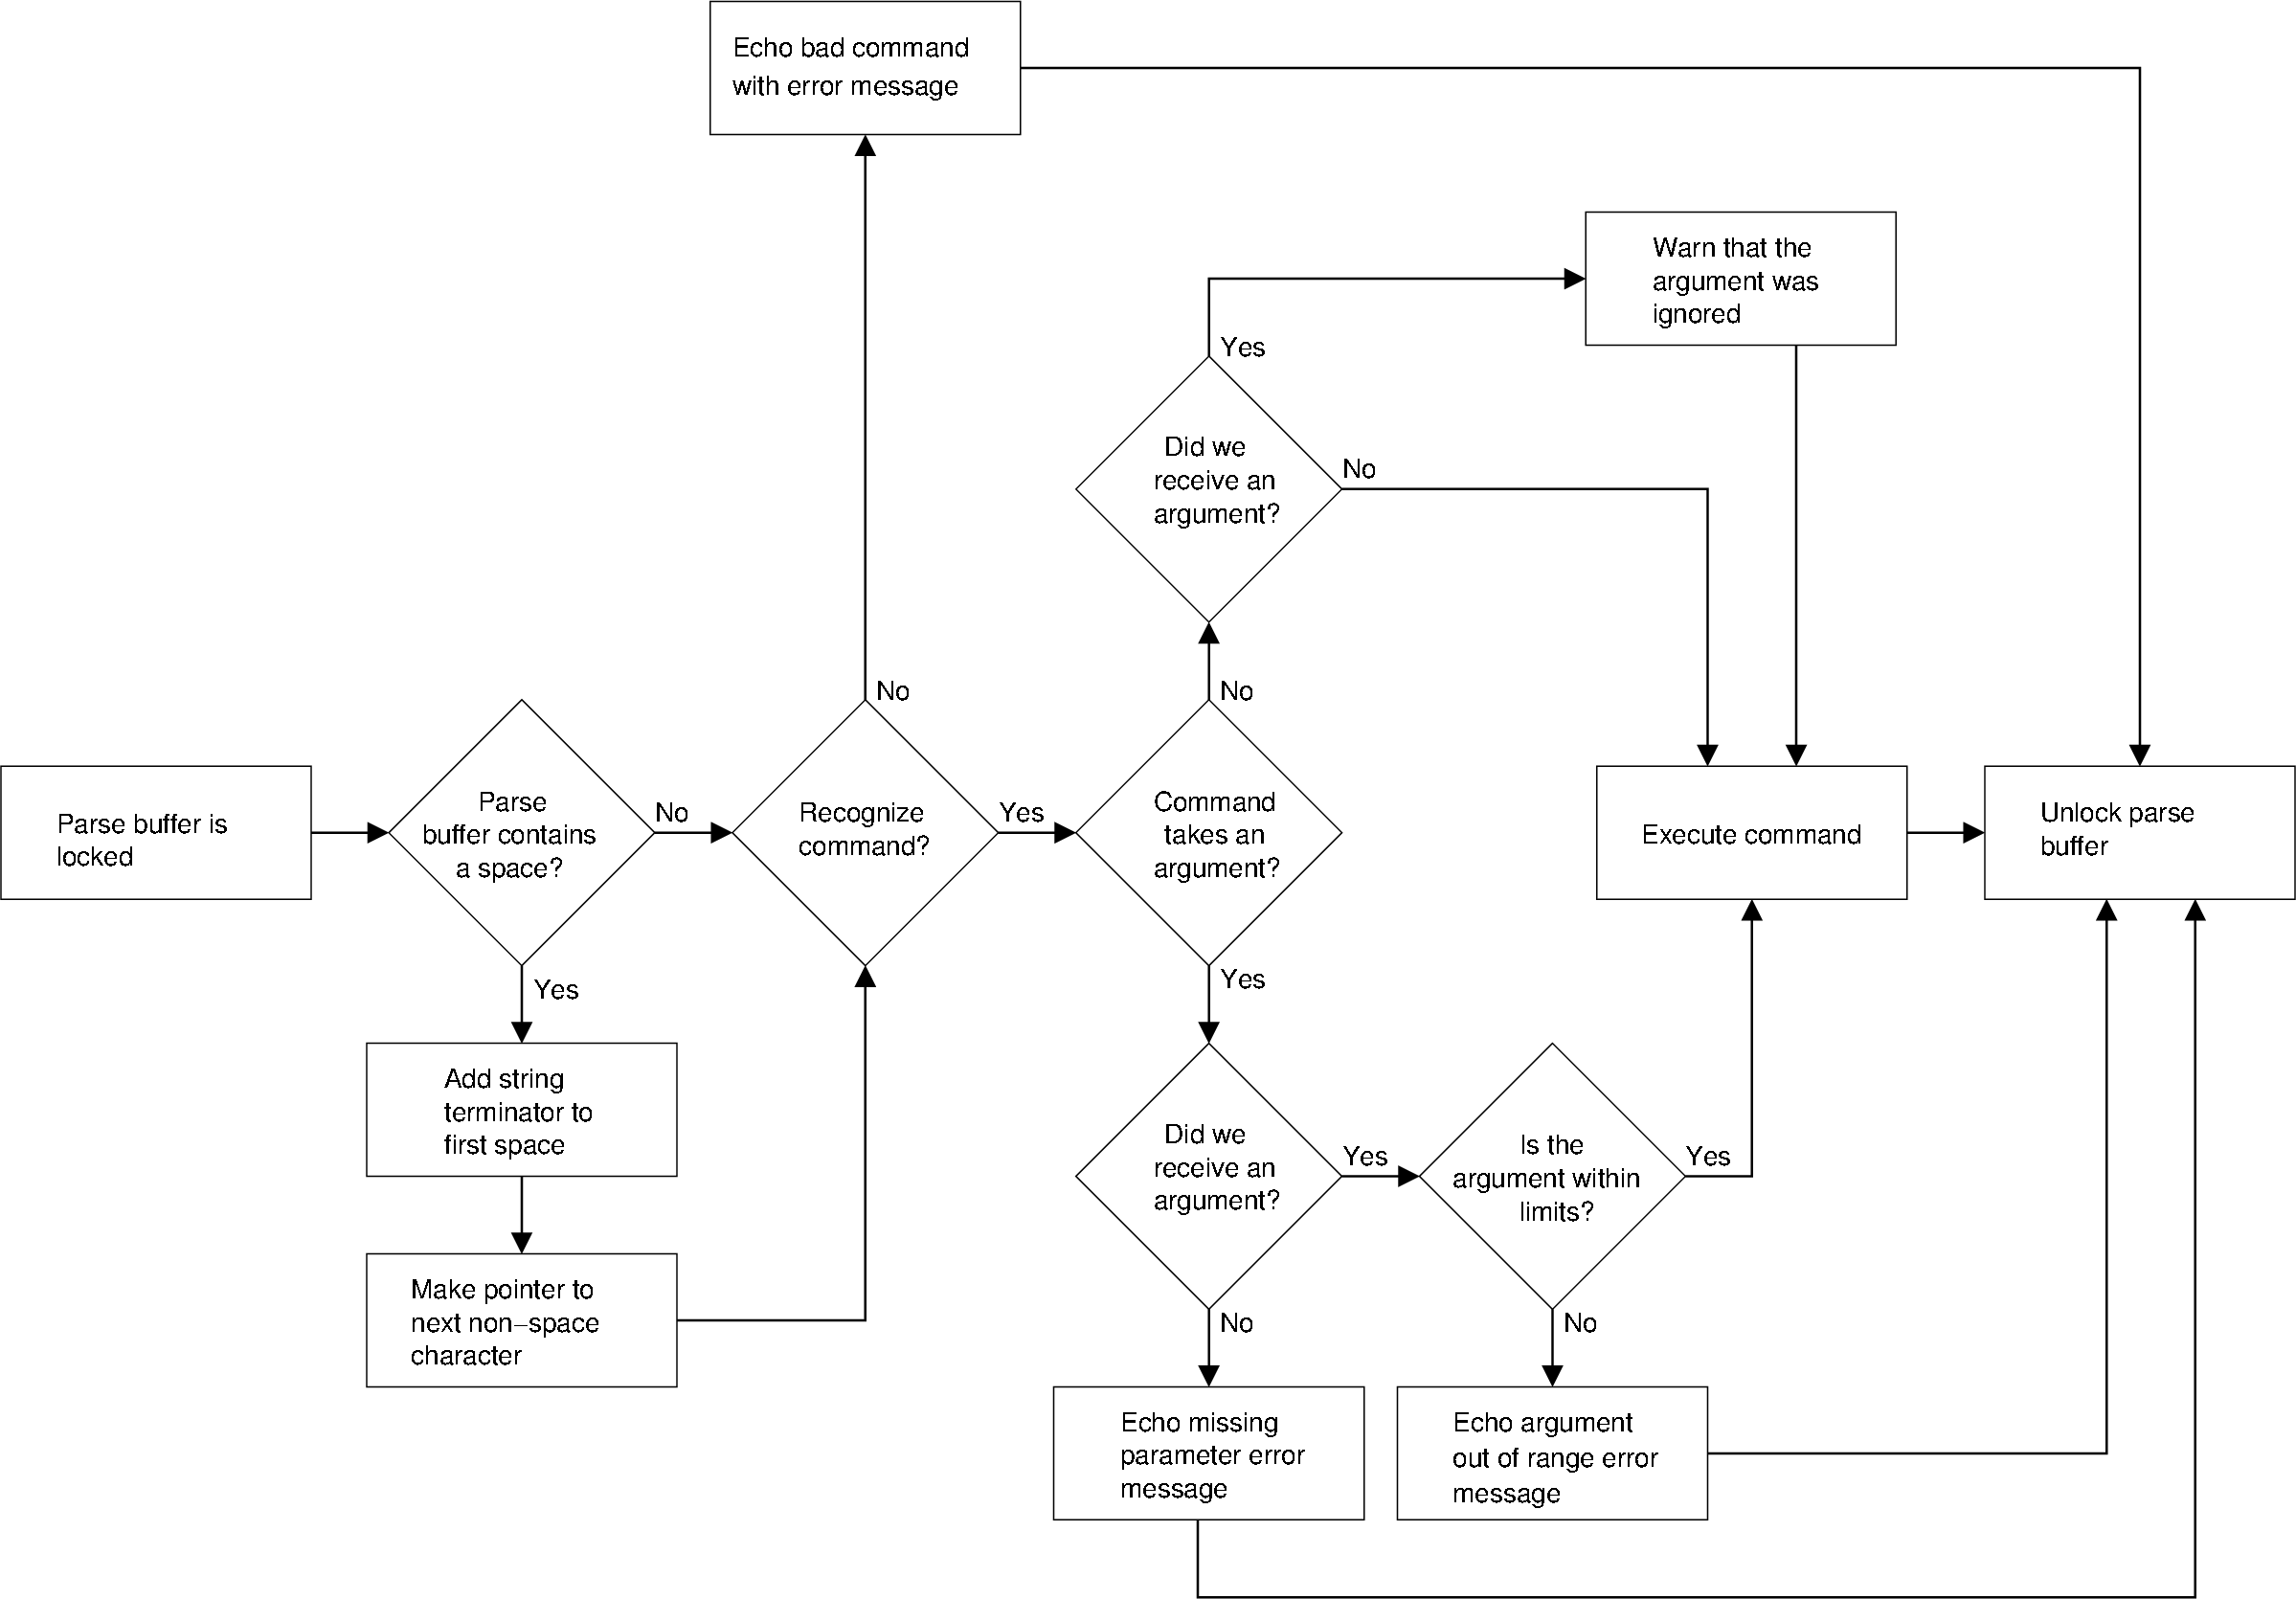
\includegraphics[clip,scale=0.5]{parse_cmd_flow}
        \caption{Program flow for processing fully-formed commands.\label{fig:cmdflow}}
    \end{center}
\end{figure}




\bibliography{doctools/latex/hydrorefs}
\end{document}
